\section{Arithmetic}
The first step in finding a balanced arithmetic was finding a scheme for the balancing of the individual values.
While the general shape of the scheme was pretty much clear from the start, the location of $x$ and $\bar{x}$ emerged during my work on the balanced operation.
\Cref{fig:schemes} shows the two schemes that are used in my project.

\begin{figure}[h]
  \centering
  \begin{subfigure}{.49\linewidth}
    \centering
    \tikzbox{scheme1.tex}
    \caption{Balancing Scheme 1}
    \label{fig:scheme1}
  \end{subfigure}
  \begin{subfigure}{0.49\linewidth}
    \centering
    \tikzbox{scheme2.tex}
    \caption{Balancing Scheme 2}
  \end{subfigure}
  \caption{Balancing Schemes}
  \label{fig:schemes}
\end{figure}

In my theoretical work I found balanced operations for both schemes, but in the end decided to use Scheme 1 because it exhibits nicer behaviour for shifts, especially rotations.
Both are worth mentioning however, because many of my operations will result in values formatted in Scheme 2 and require explicit transformation.
By having explicit ``names'' for both schemes and finding standardized transformations in both directions I could simplify the process of finding the balanced arithmetic.

\subsection{Finding Balanced Operations}
\label{operations}
After fixing the balancing scheme I started working on finding balanced variants for the binary operations in \ir{}.
Unfortunately most operations do not preserve balancedness over all intermediate steps.
They do however decrease the signal-to-noise ration for an attacker.
A more detailed analysis can be found in \Cref{balance-eval}.

\subsubsection{Scheme 1 to Scheme 2}
For better reusability I wrote down the transformations between the schemes once, and then referenced this transformation.
I thought this a better solution than implicitly including these transformations in multiple operations.

The transformation from Scheme 1 to Scheme 2 is shown in \Cref{lst:s12}.

\begin{lstlisting}[caption={Transforming from Scheme 1 to Scheme 2}, label=lst:s12]
  %1 = 00 | ~x | 00 |  x
  %2 = ~x | ~x |  x |  x                | << 8
  %3 = ~x | 00 | 00 |  x                | & 0xff0000ff
\end{lstlisting}

\subsubsection{Scheme 2 to Scheme 1}
The other direction works very similar to the first, it is shown in \Cref{lst:s21}.
Note that ROR is the ARM assembly instruction for rotational right shift, i.e. the values shifted out on the right are shifted back in on the left.

\begin{lstlisting}[caption=Transforming from Scheme 2 to Scheme 1, label=lst:s21]
  %1 = ~x | 00 | 00 |  x
  %2 = ff | ~x | 00 |  x                | ROR 24
  %3 = 00 | ~x | 00 |  x                | & 0x00ff00ff
\end{lstlisting}

\subsubsection{ORR}
Before finding a balanced variant of binary or, I needed to find an expression for the inverse of the result.
For this I utilized DeMorgan's law $\neg{x \lor y} = \neg{x} \land \neg{y}$.

\begin{lstlisting}[caption=Balanced ORR, label=lst:orr]
  %1 = 00 | ~x | 00 | x
  %2 = 00 | ~y | 00 | y
  %3 = 00 | ~x ORR ~y | 00 | x ORR y    | %1 ORR %2
  %4 = 00 | ~x AND ~y | 00 | x AND y    | %1 AND %2
  %5 = ~x AND ~y | 00 | x AND y | 00    | %3 << 8
  %6 = ~x AND ~y | ~x ORR ~y | x AND y | x ORR y   | %3 ORR %5
  %7 = ~(x ORR y) | 00 | 00 | x ORR y   | & 0xff0000ff
  %8 = 00 | ~(x ORR y) | 00 | x ORR y   | transform_2_1(%7)
\end{lstlisting}

\subsubsection{AND}
As $\neg{x \land y} = \neg{x} \lor \neg{y}$ AND works almost the same as ORR, but uses different parts of the intermediate results.

\subsubsection{XOR}
XOR is at its base a combination of AND and ORR: $x \oplus y = (\neg{x} \land y) \lor (x \land \neg{y})$.
As both balanced ORR and balanced AND have the same imbalanced intermediate values it is better to balance XOR from scratch instead of compositioning it.
The inverse of the result can be found through repeated application of DeMorgan's law and simplification.
I will skip the details of this simple transformation.
The result is: $\neg{x \oplus y} = (x \land y) \lor (\neg{x} \land \neg{y})$.

My version of balanced XOR already includes some ARM specific optimizations.
In ARM shift operations happen in a so-called barrel shifter, and can be applied to the right-hand argument of any other instruction.
I utilize this property in my balanced version of XOR to save some unnecessary cycles.

\begin{lstlisting}[caption=Balanced XOR, label=lst:xor]
  %1 = 00 | ~x | 00 |  x
  %2 = 00 | ~y | 00 |  y
  %3 = ~x | ~x |  x |  x              | %1 ORR (%1 << 8)
  %4 =  y | ~y | ~y |  y              | %2 ORR (%2 ROR 8)
  %5 = ~x AND y | ~x AND ~y | x AND ~y | x AND y   | %3 AND %4
  %6 = x XOR y | ~(x XOR y) | x XOR y | ~(x XOR y)   | %5 AND (%5 ROR 16)
  %6 = ~(x XOR y) | x XOR y | ~(x XOR y) | x XOR y   | %6 ROR 8
  %7 = ~(x XOR y) | 00 | 00 | x XOR y   | %7 & 0xff0000ff
  %8 = transform_2_1(%7)
\end{lstlisting}

\subsubsection{ADD}
For the inverse of arithmetic operations I utilized the definition of the negation in 2s complement: $-x = \neg{x} + 1$.
This also means that $\neg{x} = -x - 1$ and therefore:
\begin{equation*}
  \neg{x + y} = - (x + y) - 1 = - x - y - 1 = \neg{x} + 1 + \neg{y} \cancel{+ 1} \cancel{- 1} = \neg{x} + \neg{y} + 1
\end{equation*}

Using associativity of addition the balanced variant of ADD looks like the following:
\begin{align*}
  \%1 &= 0 && \bsep \neg{x} &&\bsep 0 &&\bsep x      &&\\
  \%2 &= 0 && \bsep \neg{y} &&\bsep 0 &&\bsep y      &&\\
  \%3 &= 0 && \bsep \neg{x}+1 &&\bsep 0 &&\bsep x    &&\;|\ \%1 + \hex{00010000}\\
  \%4 &= c && \bsep \neg{x+y} &&\bsep c' &&\bsep x+y &&\;|\ \%3 + \%2\\
  \%5 &= 0 && \bsep \neg{x+y} &&\bsep 0 &&\bsep x+y  &&\;|\ \%4 \land \hex{00ff00ff}
\end{align*}
Both $c$ and $c'$ denote possible carry bits that need to be filtered.

\subsubsection{SUB}
For subtraction I again use the definition of 2s complement, giving me the following for the inverse result:
\begin{equation*}
  \neg{x-y} = - (x-y) - 1 = y - x - 1 = y + (-x -1) = y + \neg{x} = \neg{x} + y
\end{equation*}
Applying the same definition to the regular result yields
\begin{equation*}
  x-y = x + \neg{y} + 1
\end{equation*}
resulting in a quick and convenient balanced subtraction:
\begin{align*}
  \%1 &= 0 && \bsep \neg{x} &&\bsep 0 &&\bsep x      &&\\
  \%2 &= 0 && \bsep \neg{y} &&\bsep 0 &&\bsep y      &&\\
  \%3 &= 0 && \bsep y &&\bsep 0 &&\bsep \neg{y}    &&\;|\ \%2 \ror 16\\
  \%4 &= 0 && \bsep y &&\bsep c &&\bsep \neg{y}+1 &&\;|\ \%3 + \hex{00000001}\\
  \%5 &= c' && \bsep \neg{x}+y &&\bsep c'' &&\bsep x+\neg{y}+1  &&\;|\ \%1 + \%4\\
  \%6 &= 0 && \bsep \neg{x-y} &&\bsep 0 &&\bsep x-y &&\;|\ \%5 \land \hex{00ff00ff}
\end{align*}

\subsubsection{MUL}
The inverse result of multiplication can be calculated as follows:
\begin{equation*}
  \neg{x \cdot y} = -(x \cdot y) - 1 = (-x) \cdot y - 1 = (\neg{x} + 1) \cdot y = \neg{x} \cdot y + y - 1
\end{equation*}

Which gives us the following balanced multiplication:
\begin{align*}
  \%1 &= 0 && \bsep \neg{x} && \bsep 0 && \bsep x &&\\
  \%2 &= 0 && \bsep \neg{y} && \bsep 0 && \bsep y &&\\
  \%3 &= \neg{y} && \bsep 0 && \bsep 0 && \bsep y &&\;|\ \trans21(\%2)\\
  \%4 &= c && \bsep \neg{x} \cdot y && \bsep c' && \bsep x \cdot y &&\;|\ \%1 \cdot \%3\\
  \%5 &= c'' && \bsep \neg{x \cdot y} + 1 && \bsep c' && \bsep x \cdot y &&\;|\ \%4 + (\%2 << 16)\\
  \%6 &= c''' && \bsep \neg{x \cdot y} + 1 && \bsep c' && \bsep x \cdot y &&\;|\ \%5 + \hex{00ff0000}\\
  \%7 &= 0 && \bsep \neg{x \cdot y} + 1 && \bsep 0 && \bsep x \cdot y &&\;|\ \%6 \land \hex{00ff00ff}
\end{align*}

Practical evaluation shows that computing multiplication via repeated balanced addition shows better balancing properties (see \Cref{balance-eval}) than the direct variant, so I used that for my thesis.

\subsubsection{DIV and REM}
Just like multiplication, I used repeated balanced subtraction for DIV (division) and REM (remainder) operations.
The code was written in C and can be found in the git of my thesis\cite{git}.

\subsubsection{Shifting}
When performing logical shifts, I need to ensure that the correct bits are pushed in.
As 0s are shifted in for $x$ I have to shift in 1s for $\neg{x}$.
This means that I have to ORR \hex{ff000000} for right shifts and \hex{0000ff00} for left shifts.
The shifting is performed normally and the result is then AND filtered with \hex{00ff00ff} to comply with Scheme 1 again.

\subsection{Testing for Correctness}
Before I started implementing my balancing pass I wanted to verify the correctness of my arithmetic.
For this purpose I wrote python code to calcuate all operations step by step while saving the intermediate results.
\Cref{lst:multiop} shows the intermediate steps for addition.

\begin{lstlisting}[language=python, caption=Step-by-step execution of balanced multiplication, label=lst:multiop]
m = MultiStepOperation([
    Convert_1_2(1), #2
    BinaryOperation(0,2, lambda x,y: (x*y) & 0xffffffff),#3
    BinaryOperation(3,1, lambda x,y: x + (y << 16)), #4
    UnaryOperation(4, lambda x: x + 0x00ff0000), #5
    UnaryOperation(5, lambda x: x & 0x00ff00ff), #6
])
\end{lstlisting}

The \emph{Unary-} and \emph{BinaryOperation} classes take the indices of the layers to operate on (0 and 1 are the inputs, all others are intermediate values), as well as the operation in form of a lambda.
Executing the \emph{MultiStepOperation} will then execute all lambdas in order and store the intermediate results in \emph{numpy} arrays.
After the execution there are $2^8 \cdot 2^8 = 2^{16}$ intermediate results for each operation (the inputs only have $2^8$ values each).
Correctness is then tested by checking if all final results are equal to the output of a function to compare to ($x \cdot y$ in this case).

\subsection{Evaluating the Balancedness}
\label{balance-eval}
Balancedness of my operations is evaluated using the same python code.
As all intermediate results are stored during evaluation I can easily calculate the distribution of their \hammingw s, as shown in \Cref{fig:mult}.
I used these histograms to check if operations needed improvement, and if that was the case, I tried to find a different, more balanced way of performing them.

\begin{figure}[h]
  \centering
  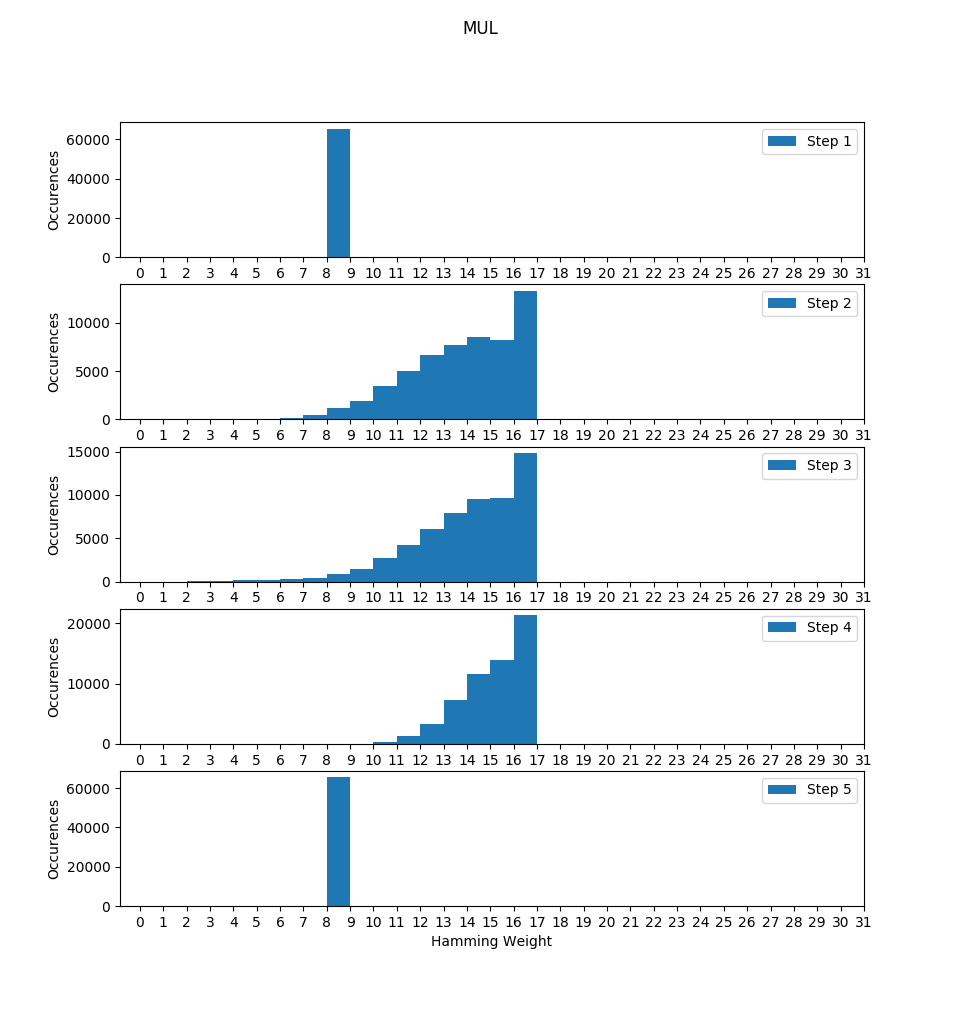
\includegraphics[width=\textwidth]{multiplication.png}
  \caption{Histogram of \hammingw s of direct balanced multiplication}
  \label{fig:mult}
\end{figure}

\Cref{fig:mult} also shows that while directly computing multiplication is balanced for a lot of values, it still leaks information in almost every step.
For this reason I implemented it as repeated addition in my pass.
